\chapter{Transporting safe continuation through a quotient}\label{ch:controltransport}

The previous chapters establish a stochastic quotient and a safe-ending game separately. To use both in one system, the retained state must also preserve the successor choices relevant to a sure guarantee. Probabilities and supports have different roles here. A small positive transition probability still creates a possible path. It cannot be discarded in a claim that quantifies over every path.

This chapter gives an exact interface between representation change and the two fixed-point constructions. It then weakens equality to a one-sided enclosure that can certify an entire family of models.

\section{The controlled predecessor}
Let $X,Z$ be finite nonempty sets and $\pi:X\to Z$ a surjection. Use a common finite action alphabet with separate running and ending catalogues $A^X_m(x)$ and $A^Z_m(z)$, where $m\in\{\mathrm{run},\mathrm{end}\}$. Every admitted action has a nonempty successor set. The mode can be included in the action name, so the same printed action in two modes need not denote the same transition.

Assume the fine and coarse safe and goal sets agree by inverse image:
\[
 S_X=\pi^{-1}(S_Z),\qquad G_X=\pi^{-1}(G_Z),\qquad G_Z\subseteq S_Z.
\]
This is a substantive restriction. A label that distinguishes a safe state from an unsafe state cannot be omitted from a safety-preserving quotient.

For $B\subseteq X$, define the mode-specific predecessor
\[
 \operatorname{CPre}^X_m(B)
 =\{x:\exists a\in A^X_m(x),\ \operatorname{Post}_X(x,a)\subseteq B\}.
\]
Define $\operatorname{CPre}^Z_m$ in the same way. These operators do not themselves include a safety test. Safety enters the ending recurrence through its intersection with $S$, and the running recurrence through its current set.

\begin{lemma}[Predecessors commute with an exact controlled quotient]\label{r:control-predecessor}
Suppose, for each mode and fine state,
\begin{align*}
 A^X_m(x)&=A^Z_m(\pi x),\\
 \pi(\operatorname{Post}_X(x,a))&=\operatorname{Post}_Z(\pi x,a)
 \qquad(a\in A^X_m(x)).
\end{align*}
Then for every $B\subseteq Z$,
\[
 \operatorname{CPre}^X_m(\pi^{-1}B)
 =\pi^{-1}(\operatorname{CPre}^Z_m(B)).
\]
\end{lemma}
\begin{proof}
For an admitted action,
\[
 \operatorname{Post}_X(x,a)\subseteq\pi^{-1}B
 \quad\Longleftrightarrow\quad
 \pi(\operatorname{Post}_X(x,a))\subseteq B.
\]
Replace the projected successor set by its assumed coarse value. The action ranges in the two existential quantifiers are identical, so existence of a witnessing action is equivalent on both sides.
\end{proof}

\section{Transport of both fixed-point sequences}
Construct $T^X_k,L^X_k$ on the fine game and $T^Z_k,L^Z_k$ on the coarse game as in Chapter~\ref{ch:endinganalysis}. In particular, the running sequence starts from the stable ending region in its own model.

\begin{theorem}[Ending regions, running kernels, and ranks are preserved]\label{r:control-transport}
Under the exact controlled-quotient assumptions,
\[
 T^X_k=\pi^{-1}(T^Z_k),\qquad
 T^X_*=\pi^{-1}(T^Z_*),\qquad
 L^X_k=\pi^{-1}(L^Z_k),\qquad
 L^X_*=\pi^{-1}(L^Z_*)
\]
for every finite $k$. For every $x\in T^X_*$, the first-entry ranks agree:
\[
 \rho_X(x)=\rho_Z(\pi x).
\]
A positional coarse policy for safe continuation and ending lifts to a fine policy with the same rank bound. To execute that lift, the controller needs the current coarse state and command mode, but not the remaining fine-state coordinates.
\end{theorem}
\begin{proof}
The goal-set assumption gives equality at $T_0$. Inverse images commute with union and intersection. Applying Lemma~\ref{r:control-predecessor} to the ending predecessor gives the induction step
\begin{align*}
 T^X_{k+1}
 &=T^X_k\cup\bigl(S_X\cap\operatorname{CPre}^X_{\rm end}(T^X_k)\bigr)\\
 &=\pi^{-1}\!\left(T^Z_k\cup
       (S_Z\cap\operatorname{CPre}^Z_{\rm end}(T^Z_k))\right).
\end{align*}
The finite increasing sequences stabilize, so their stable sets also agree by inverse image. The first stage at which $x$ appears is exactly the first stage at which $\pi x$ appears, proving rank equality.

The equality of stable ending sets gives the base of the running induction. The recurrence is intersection with the running predecessor. The same inverse-image calculation proves equality at every running stage and hence at stabilization.

At a coarse state in $L^Z_*$, choose a running action whose successors remain in that set. It is admitted at every fine representative, and all its fine successors lie in $\pi^{-1}(L^Z_*)=L^X_*$. After the command, choose a coarse ending action that decreases rank. Its projected successors have smaller coarse rank, so every fine successor has smaller fine rank. These choices define the lifted policy.
\end{proof}

The equality is stronger than soundness of one selected policy. A fine state is winning exactly when its coarse image is winning, even if a proposed fine policy uses additional hidden coordinates. Chapter~\ref{ch:endinganalysis} characterizes all winning states through the fixed points, including those achievable by history-dependent policies. An exact quotient therefore does not conceal a better sure-ending strategy that depends on discarded state.

This does not give the controller an observation it did not have. A report-only policy from Chapter~\ref{ch:jointcontract} need not know its current coarse state. Applying the policy-lifting conclusion requires that $\pi x$ be observed or reconstructed from an available record. Equality of the abstract winning regions alone does not solve a partially observed control problem.

\section{From stochastic rows to successor supports}
Suppose a mode's game successors are exactly the support of the stochastic instrument:
\[
 \operatorname{Post}_X(x,a)
 =\{x':\exists o,\ K_{a,o}(x'\mid x)>0\}.
\]
Define the coarse successor set from $\bar K$ in the same way.

\begin{corollary}[An exact stochastic quotient preserves the support game]\label{r:stochastic-support-game}
The joint quotient of Theorem~\ref{r:joint-quotient} gives
\[
 \pi(\operatorname{Post}_X(x,a))=\operatorname{Post}_Z(\pi x,a)
\]
for every enabled action. If the mode catalogues and the safe and goal sets satisfy the preceding compatibility conditions, Theorem~\ref{r:control-transport} applies to the resulting support games.
\end{corollary}
\begin{proof}
For each $o,z'$, the coarse entry is a finite sum of nonnegative fine entries. It is positive exactly when at least one fine successor in that fibre has a positive entry for that report. Taking the union over reports gives the support identity. Normalization makes the support of every enabled action nonempty. The remaining hypotheses are precisely those of Theorem~\ref{r:control-transport}.
\end{proof}

A sure guarantee in this support game covers all supported successor paths. It is stronger than almost-sure success under a probability law. An infinite path can have probability zero while every one of its finite prefixes has positive probability. The support-game interpretation deliberately retains that path.

\section{Conservative enclosures give one-sided certificates}
Exact equality is not needed to certify a policy conservatively. Suppose instead that a coarse envelope admits only actions available at every fine representative and includes all projected actual successors:
\[
 A^Z_m(\pi x)\subseteq A^X_m(x),\qquad
 \pi(\operatorname{Post}_X(x,a))
 \subseteq\operatorname{Post}_Z(\pi x,a)
 \quad(a\in A^Z_m(\pi x)).
\]
The envelope may contain additional adverse successors and may omit some fine actions. Retain the exact inverse-image assumptions for safety and goals.

\begin{proposition}[A winning envelope policy remains winning]\label{r:control-envelope}
Under these one-sided assumptions,
\[
 \pi^{-1}(T^Z_*)\subseteq T^X_*,\qquad
 \pi^{-1}(L^Z_*)\subseteq L^X_*.
\]
A coarse ending rank bounds the ending time of the lifted policy. The same coarse policy works for every fine model satisfying the enclosure assumptions. The reverse inclusions need not hold.
\end{proposition}
\begin{proof}
Induction on the coarse ending stages proves
$\pi^{-1}(T^Z_k)\subseteq T^X_k$. A witnessing coarse action is available at each fine representative. Its actual successors project into the envelope's successors and hence into the previous coarse stage. The fine action therefore witnesses the next fine stage. The same argument proves rank decrease along every lifted ending path.

The inverse image of $L^Z_*$ lies inside $T^X_*$ by the first inclusion. Choose the coarse invariant running action at each coarse state. Every fine successor lies in the inverse image of $L^Z_*$. Thus that inverse image is a controlled invariant subset of the fine ending region. The greatest-invariant characterization places it inside $L^X_*$. The argument uses only the enclosure relations and therefore applies to every model satisfying them.
\end{proof}

A conservative rejection is not a proof that the fine problem is impossible. For example, a coarse envelope may include an unsafe successor that the actual fine model never reaches. The envelope can then reject a state from which the actual model has an immediate safe ending. The conclusion is intentionally one-sided.

\section{Why a small probability error is not a sure guarantee}
Take three states $s,g,b$, with safe set $\{s,g\}$ and goal $\{g\}$. Running holds $s$ or $g$ in place. The nominal ending action at $s$ moves to $g$ with probability one. The perturbed action instead moves to $g$ with probability $1-\epsilon$ and to unsafe state $b$ with probability $\epsilon$, where $0<\epsilon<1$. A hold action is available at $g$.

The row total variation distance is exactly $\epsilon$. In the nominal game, $s$ belongs to both the ending region and the running kernel. In the perturbed support game, the only ending action from $s$ has an unsafe successor, so $s$ belongs to neither. This happens for every positive $\epsilon$, however small.

\begin{figure}[htbp]\centering
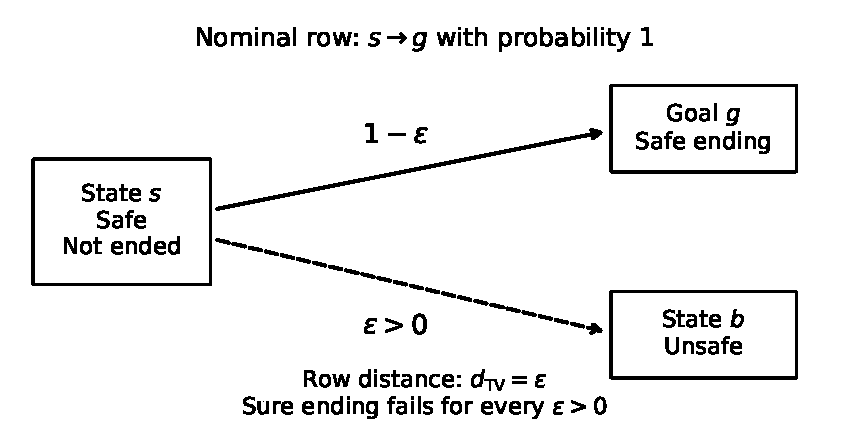
\includegraphics[width=.91\linewidth]{figures/support_margin.pdf}
\caption{An arbitrarily small unsafe branch changes a sure-ending certificate. The nominal and perturbed rows are exact declared distributions. Total variation controls probability discrepancy, not the disappearance of a supported adverse path.}\label{fig:support-margin}
\end{figure}

The appropriate robust certificate is an enclosure containing every possible successor, together with an action that succeeds throughout that enclosure. A small numerical residual is useful evidence for other purposes, but it cannot replace that quantified condition.

\section{The resulting integration}
We can now state the connection without changing the meaning of any interface. The stochastic quotient preserves controlled history laws. Its nonnegative rows induce an exact quotient of support games. Compatible safety and target labels then preserve the ending attractor, running kernel, and first-entry rank. Implementing the coarse policy still requires access to its current coarse state. Keeping these conditions separate is what makes the combined statement usable.
